%\chapter{Introduction}
%already present in the main file

\graphicspath{{../img/ch10/}}


Four relatively separate topics are presented in the present thesis and the discipline of Information Extraction is the central point of them. Each topic represents one particular aspect of the Information Extraction discipline.

The first two topics are focused on our information extraction methods based on deep language parsing. The first topic relates to how deep language parsing was used in our first method in combination with manually designed extraction rules.

The second topic deals with an alternative extraction method based on machine learning. An inductive procedure was developed based on Inductive Logic Programming (ILP), which allows automated learning of extraction rules from a learning collection.

The idea of the Semantic Web was the strongest motivation of our research from the very beginning. We wanted to exploit information extraction techniques to speed up the semantic web evolution. The third topic of the thesis presents even more than that. The core of the extraction method was experimentally reimplemented using semantic web technologies. Therefore not only the result of information extraction but also the extraction procedure itself is realized using semantic web technologies. The main advantage of this approach is the possibility to save the extraction rules in so called shareable extraction ontologies.

The last topic of this thesis is the most distant from the original information extraction topic. We have included it because it represents an important part of our research and considerable effort was spent on it. The topic deals with document classification and fuzzy logic. We are investigating the possibility of using information obtained by information extraction techniques to document classification. Our implementation of so called Fuzzy ILP Classifier was experimentally used for the purpose of document classification.

\section{Motivation}
The basic motivation of our research can be illustrated with three images or schemas that are presented in Figures~\ref{fig:acquisitions_annotated}, \ref{fig:fireman_annotated} and \ref{fig:intro_damage_tree}. The first two figures show some texts with several pieces of information decorated in it. If you show such images to a human, he or she will be shortly able to find such pieces of information in any other text of the same kind. But can this relatively simple task do a computer as well? Figure~\ref{fig:intro_damage_tree} represents our first ideas when we started to look for the answer. The figure shows a linguistic tree obtained by automated linguistic analysis of the last sentence of the second figure (Figure~\ref{fig:fireman_annotated}). It already contain lots of indications (decorated with orange tags) of where to look for the wanted piece of information, in this case, the amount of 8,000 Czech Crowns representing the total damage sought by the accident reported in the text.


\begin{figure}
\centering
\framebox{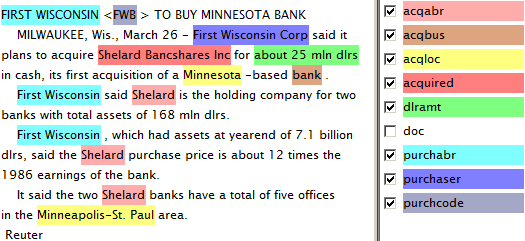
\includegraphics[width=0.75\hsize]{acquisitions_annotated}}
\caption{Annotations of Corporate Acquisition Events}
\label{fig:acquisitions_annotated}
\end{figure}


\begin{figure}
\centering
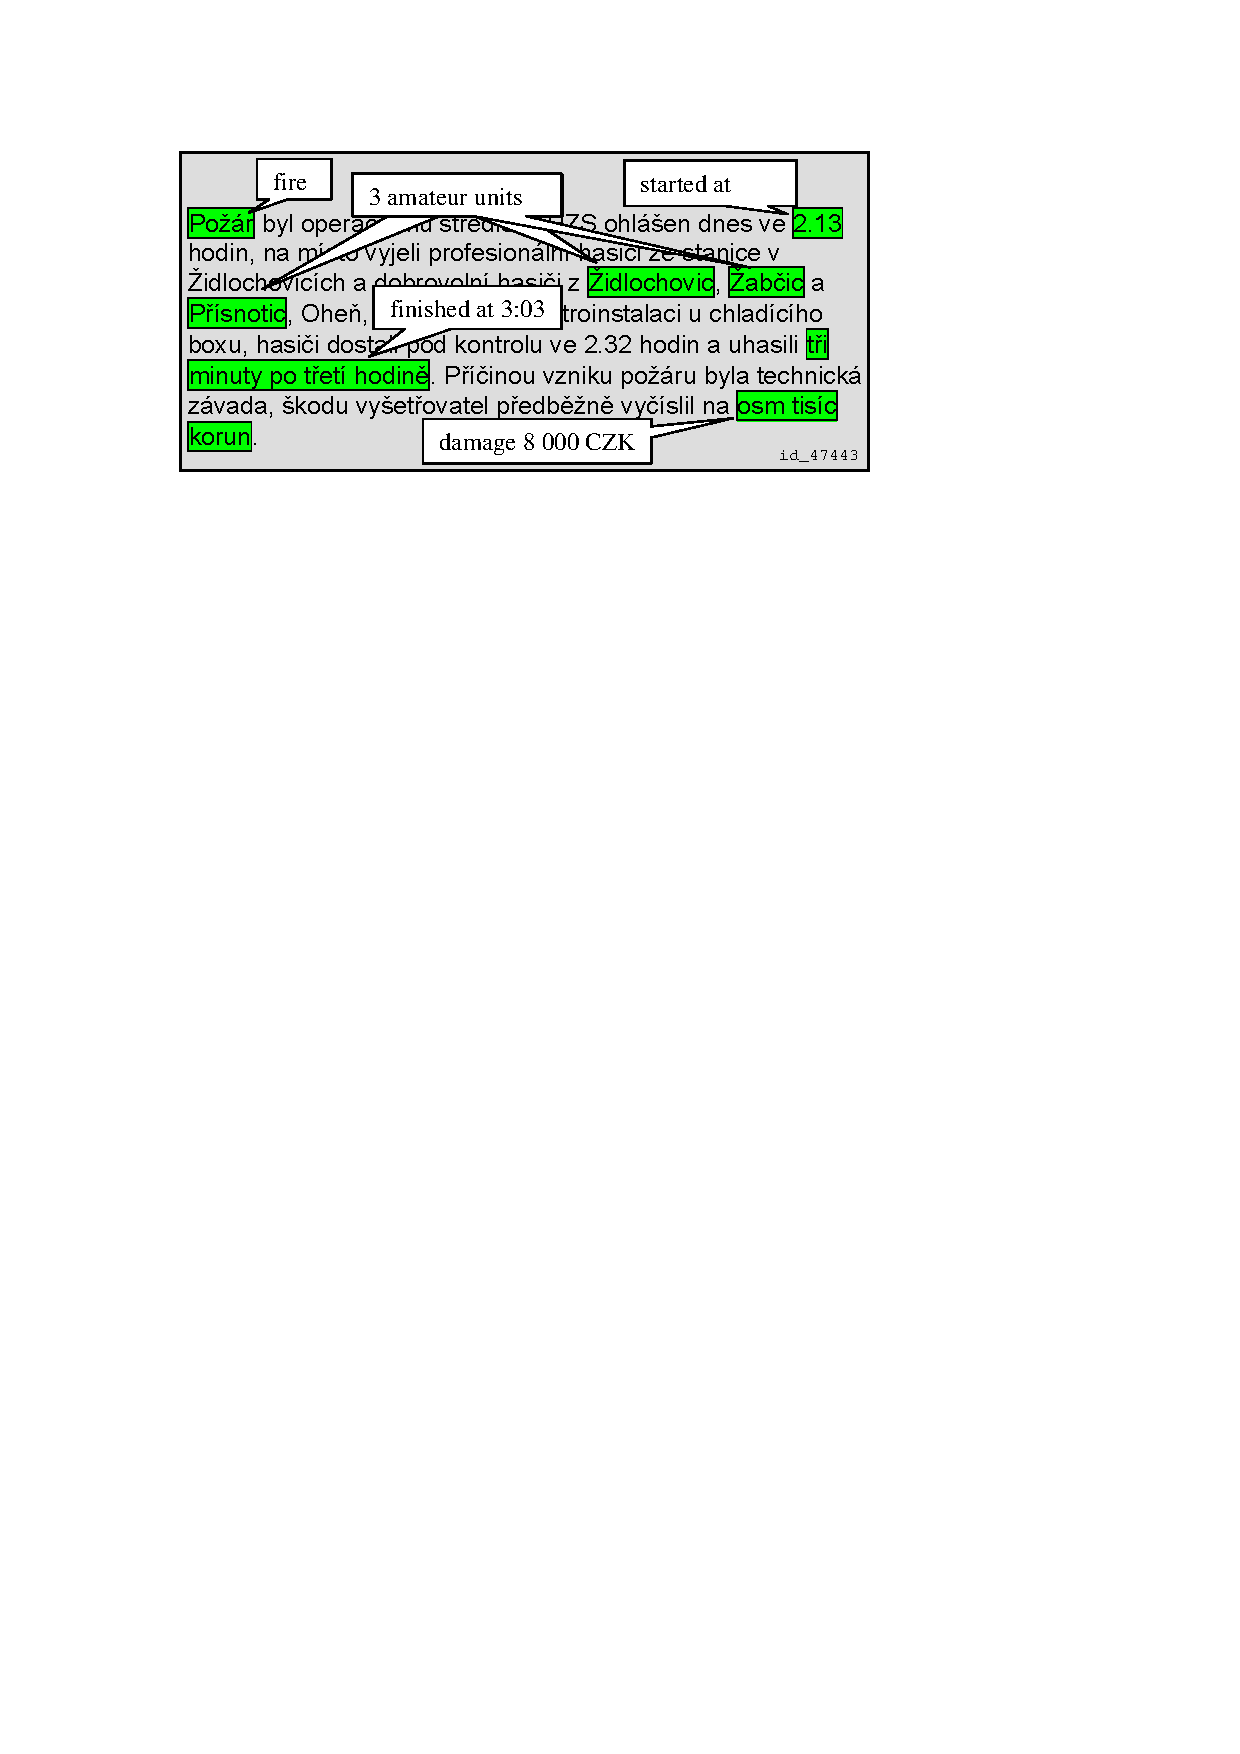
\includegraphics[width=0.65\hsize]{fireman_annotated}
\caption{Annotations of Czech Fireman events}
\label{fig:fireman_annotated}
\end{figure}


\begin{figure}
\centerline{\framebox{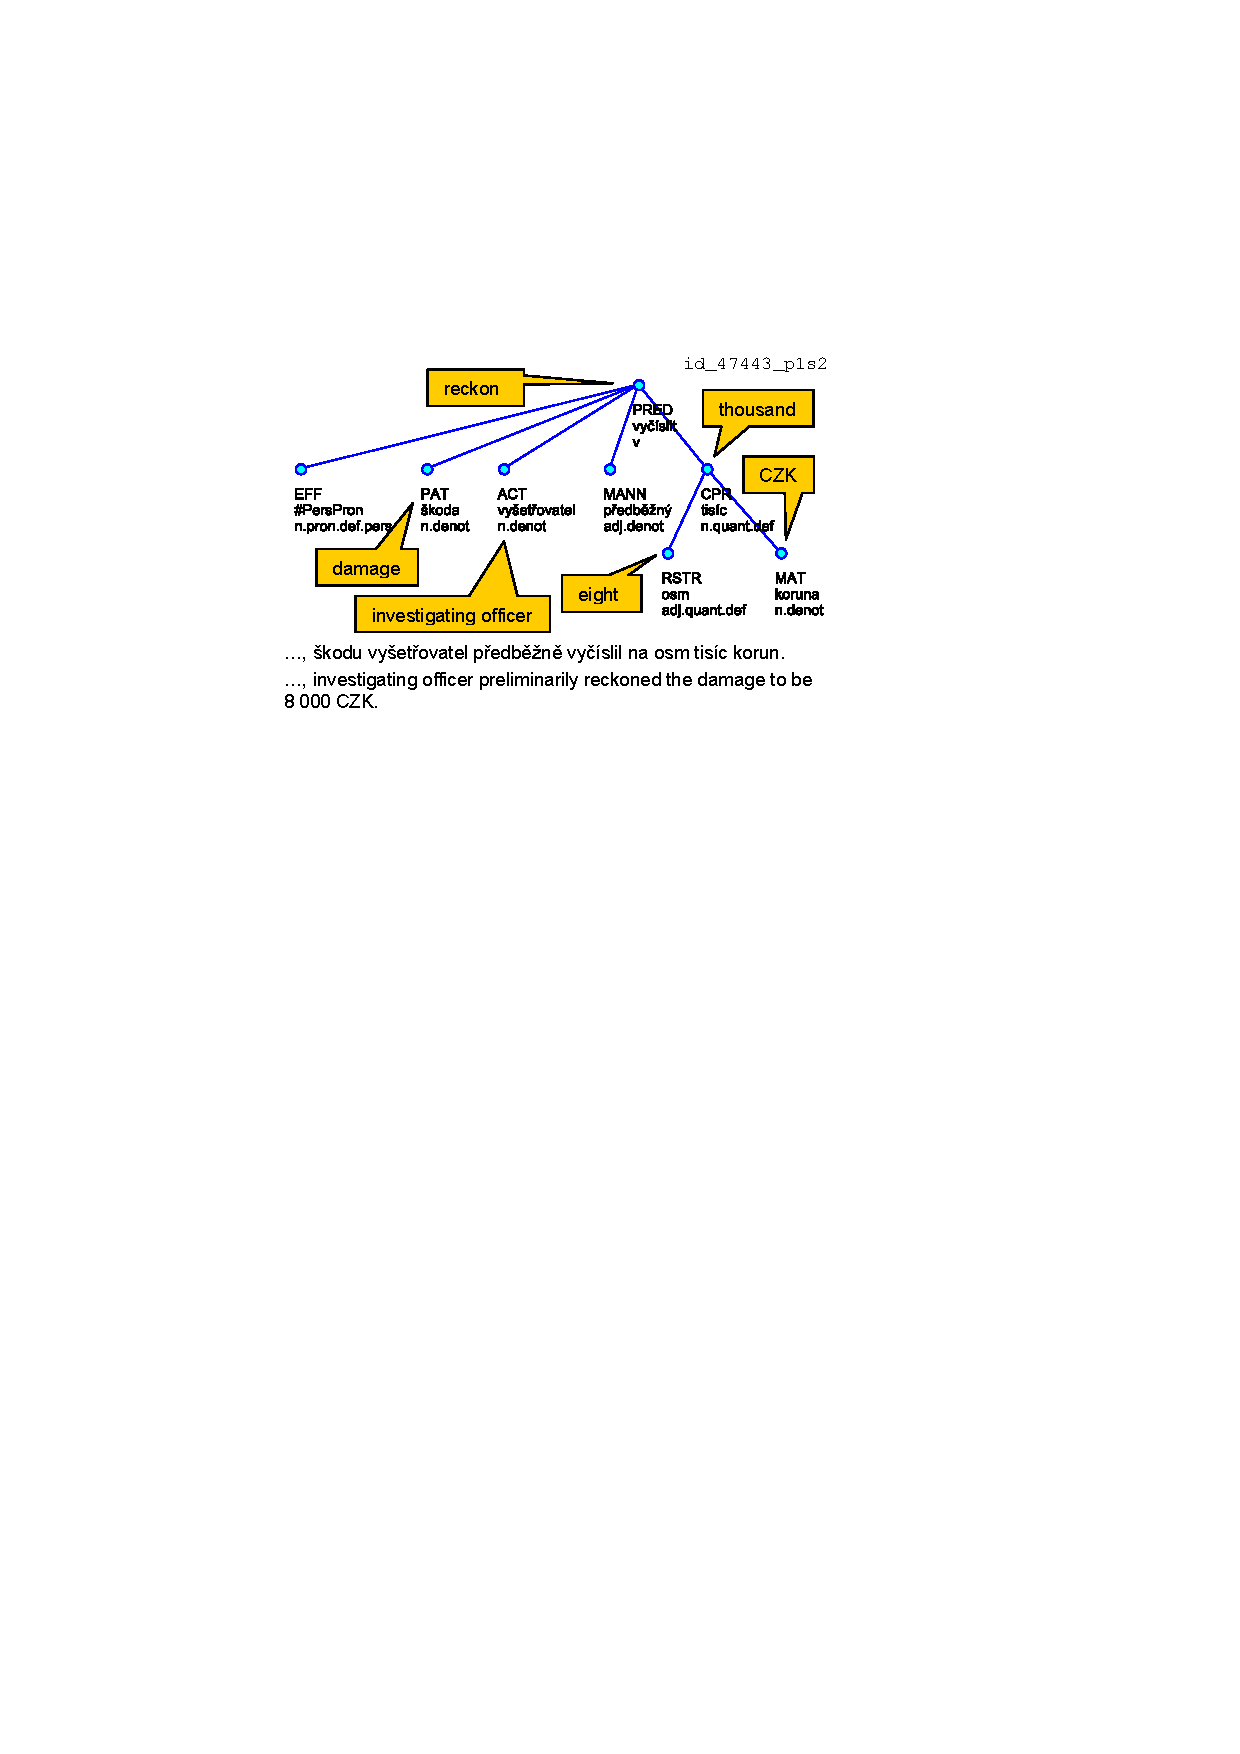
\includegraphics[width=0.7\hsize]{damage_tree}}}
\caption{Example of a linguistic tree of one analyzed sentence.}
\label{fig:intro_damage_tree} 
\end{figure}


%\subsection{Motivation of Our Approaches}

The main motivation for creating our extraction methods was an attempt to use deep linguistic analysis for this task. Especially for the Czech language with free word order this seemed reasonable. It is much more straightforward to design extraction rules on the basis of linguistic dependency trees than to struggle with the surface structure of text. In a dependency tree, the position of a word is determined by its syntactic (analytical trees) or even semantic role (tectogrammatical trees). So the extraction rules might not be dramatically affected by minor variations of the word order.

%\subsection{Usage}
Besides that information extraction and annotation is very interesting and challenging problem, it is also particularly useful. This period can be characterized by information overload and information extraction can provide partial answer to that. It provides fine grained indexing of documents, which supports precise search and document filtering. Navigation within individual documents can be faster and reading can be more effective. Other software programs can use the extracted information and perform additional computations resulting in summaries and answers integrated from different sources.  The effort in this direction will hopefully culminate in the realization of the idea of the Semantic Web, when all the information will be available in a machine workable form and the whole (semantic) web could be used as a huge knowledge base.



\section{Main Contributions} \label{sec:phd_contributions}

Let us briefly summarize the main contributions of the present work.

\subsection{New Ideas, Models and Methods}

Novel and original approaches or adaptations of existing ones are presented in this work.

The extraction method based on manually designed extraction rules is unique in the high expressiveness of extraction rules and the existence GUI (Graphical User Interface) for graphical design of these rules, both of these benefits are brought by the existence of the linguistic tool Netgraph (Section~\ref{sec:third_netgraph}), which was exploited as the core of the extraction method.

Very similar approaches to our extraction method based on ILP were already reported in literature, but they were developed partly in parallel with our solution and they do not provide a publicly available and usable implementation. The method also represents the first attempt to use PDT (Prague Dependency Treebank) resources (e.g. tectogrammatical trees, Sections~\ref{sec:third_pdt_tools_and_resources}) in the area of information extraction. Evaluation of the method on the language pair of Czech and English demonstrates its language independence.

The topic of shareable extraction ontologies introduces completely new paradigm to the design and usage of extraction ontologies \citep{DBLP:conf/er/EmbleyTL02}. The usage of a semantic web reasoner as the interpreter of an extraction ontology has never been demonstrated before.

Last but not least, the attempt to use information extracted from a document for document classification is also reported for the first time, although our attention is more focused on the implementation and evaluation of the Fuzzy ILP Classifier based on the sound theory of fuzzy ILP.



\subsection{New Software}

As a part of our work, new publicly available implementation of the described methods was created. 

A simple and extensible API (Application Programming Interface) interface of the extraction method based on manually designed extraction rules is provided such that users can design extraction rules in the Netgraph GUI and evaluate them on the whole corpus using this interface. 

The extraction method based on ILP is fully integrated in GATE (a widely used framework for text engineering; Section~\ref{sec:third_gate}) and it can be used as any other machine learning algorithm inside the framework. Moreover integration of TectoMT linguistic tools (Section~\ref{sec:third_tectomt}) as well as the Netgraph tree viewer (Section~\ref{sec:learning_GATE_Netgraph}) to the GATE framework was realized. Our implementation also provides utility functions for  comparative information extraction experiments using the cross-validation technique and investigation of statistical significance. 

The implementation of the case study with shareable extraction ontologies is not that general as the rest of the software part of our work but it can be easily followed and reproduced in similar experiments.

The implementation of the Fuzzy ILP Classifier (Section~\ref{sec:fuzzy_impl}) is fully compatible with Weka (a widely used framework for machine learning experiments; Section~\ref{sec:third_weka}) and it can be used as any other Weka classifier, it also provides the possibility of custom integration of the classifier to an existing installation of the Weka system on the user's computer.

\subsection{New Data}

Several new datasets were established as a part of our work. See the complete list of contributed datasets in Section~\ref{sec:data_contributed}.

\subsection{Exploitation of Existing Resources}

Work of other researchers was exploited, extended and/or evaluated in the present work. For example our extraction methods represent the first application of PDT resources (e.g. Netgraph, tectogrammatical trees, etc.) in the area of information extraction. See also the description of experiments performed with the PAUM extraction algorithm (Section~\ref{sec:learning_eval_PAUM}), with various semantic web reasoners (Section~\ref{sec:onto_reasoners}), Weka classifiers (Section~\ref{sec:fuzzy_eval}), etc.

\subsection{Evaluation Experiments}

All approaches presented in this thesis were evaluated such that readers can obtain clear picture abut the performance and usability of these approaches. Most evaluation experiments are detailed and comprehensive, investigating also the statistical significance of the results.

\subsection{Publications and New Publicly Available Resources}

Majority of topics presented in this thesis were already published (going through peer review process), presented and discussed with international audience. Moreover several citations can be found in the literature showing that the work is already contributing to the generally available knowledge. See the complete list of publications in the appendix, Chapter~\ref{sec:my_publications}.

Also the software and data parts of our work are publically available on the web, Section~\ref{sec:download_notes} provides details about the availability of these resources.  


\section{Organization}

Rather than presenting individual topics or approaches of this thesis separately in distinct chapters, we decided to organize this document according to common aspects of these approaches and to dedicate individual chapters to these aspects instead of  approaches. This way, all the (four) topics are described in parallel in each chapter. 

Chapter~\ref{sec:ch_problems} provides definitions of the individual problems and consequent tasks solved later in this thesis.
Chapter~\ref{sec:ch_related} contains description of the most related work of other scientists.
Chapter~\ref{sec:ch_third_party} introduces the most important third party tools and resources that were used in our research.
Chapter~\ref{sec:ch_methods} describes solutions, used models and methods of the individual approaches presented in this thesis.
Chapter~\ref{sec:ch_implementation} provides details about implementation of all the approaches.
Chapter~\ref{sec:ch_data} describes all datasets that were used in our experiments.
Chapter~\ref{sec:ch_eval} describes all experiments that we performed mostly for evaluation of the approaches.
Finally, Chapter~\ref{sec:ch_conclusion} concludes the thesis.

